\documentclass[]{beamer}

\usepackage{pgfpages}

\setbeamertemplate{footline}[frame number]
\setbeamertemplate{navigation symbols}{}%remove navigation symbols
%\setbeameroption{show notes}
%\setbeameroption{show notes on second screen=right}

\usepackage{url}
\usepackage{cite}
%\usepackage[margin=1in]{geometry}
\usepackage[latin1]{inputenc}
\usepackage{graphicx}
\usepackage{listings}
\usepackage{caption}
\usepackage{subcaption}
\usepackage{paralist}
% uncomment to force centering of captions in IEEE
%\usepackage{subfig}

\usepackage{hyperref}
\hypersetup{
    colorlinks,
    citecolor=black,
    filecolor=black,
    linkcolor=black,
    urlcolor=black
}




\usepackage{tikz}
\usepackage{tikz-er2}
\usetikzlibrary{shapes,arrows}
\usetikzlibrary{positioning}
\usetikzlibrary{shadows}
\tikzstyle{every entity} = [top color=white, bottom color=blue!30,
                            draw=blue!50!black!100, drop shadow]
\tikzstyle{every weak entity} = [drop shadow={shadow xshift=.7ex,
                                 shadow yshift=-.7ex}]
\tikzstyle{every attribute} = [top color=white, bottom color=yellow!20,
                               draw=yellow, node distance=1cm, drop shadow]
\tikzstyle{every relationship} = [top color=white, bottom color=red!20,
                                  draw=red!50!black!100, drop shadow]
\tikzstyle{every isa} = [top color=white, bottom color=green!20,
                         draw=green!50!black!100, drop shadow]
\tikzstyle{decision} = [diamond, draw, fill=blue!20,
    text width=4.5em, text badly centered, node distance=3cm, inner sep=0pt]
\tikzstyle{block} = [rectangle, draw, fill=blue!20,
    text width=5em, text centered, rounded corners, minimum height=4em]
\tikzstyle{edge} = [draw,line,-]
\tikzstyle{line} = [draw, -triangle 45]
\tikzstyle{cloud} = [draw, ellipse,fill=red!20, node distance=3cm,
    minimum height=2em]
\tikzstyle{dot} = [draw, circle, inner sep=1pt, fill=black]
\tikzstyle{db} = [draw,
  shape=cylinder,
  aspect=0.7,
  minimum height=2.5cm,
  minimum width=1.5cm,
  left color=yellow!30,
  right color=yellow!60,
  middle color=yellow!20, % Has to be called after left color and middle color
  outer sep=-0.5\pgflinewidth, % to make sure the ellipse does not draw over the lines
  shape border rotate=90
]


\definecolor{dkgreen}{rgb}{0,0.6,0}
\definecolor{gray}{rgb}{0.5,0.5,0.5}
\definecolor{mauve}{rgb}{0.58,0,0.82}
\lstset{ %
  language=SQL,                % the language of the code
  basicstyle=\scriptsize,           % the size of the fonts that are used for the code
  numbers=none,                   % where to put the line-numbers
  numberstyle=\tiny\color{gray},  % the style that is used for the line-numbers
  stepnumber=2,                   % the step between two line-numbers. If it's 1, each line 
                                  % will be numbered
  numbersep=5pt,                  % how far the line-numbers are from the code
  backgroundcolor=\color{white},      % choose the background color. You must add \usepackage{color}
  showspaces=false,               % show spaces adding particular underscores
  showstringspaces=false,         % underline spaces within strings
  showtabs=false,                 % show tabs within strings adding particular underscores
  frame=single,                   % adds a frame around the code
  rulecolor=\color{black},        % if not set, the frame-color may be changed on line-breaks within not-black text (e.g. comments (green here))
  tabsize=2,                      % sets default tabsize to 2 spaces
  captionpos=b,                   % sets the caption-position to bottom
  breaklines=true,                % sets automatic line breaking
  breakatwhitespace=false,        % sets if automatic breaks should only happen at whitespace
  title=\lstname,                   % show the filename of files included with \lstinputlisting;
                                  % also try caption instead of title
  keywordstyle=\color{blue},          % keyword style
  commentstyle=\color{dkgreen},       % comment style
  stringstyle=\color{mauve},         % string literal style
  escapeinside={\%*}{*)},            % if you want to add LaTeX within your code
  morekeywords={*,...}               % if you want to add more keywords to the set
}

\newcommand{\pad}{\vbox to 20pt{}}


\title[]{Coexist: A Minimalist Data Access System}
\author[]{Anthony Naddeo \\ advisor: Sudarshan Chawathe}
\date{\today}

\usetheme{Berkeley}
\usecolortheme{whale}

\begin{document}

%--------------------------------------------------------
\begin{frame}
\titlepage

\note{
Hi, my name is Anthony Naddeo, my advisor is Professor Chawathe, and I am going
to present Coexist: a minimalist data access system for arbitrary client types.
}
\end{frame}


%--------------------------------------------------------
\section{The Problem}

\begin{frame}
\frametitle{The Problem}

\begin{itemize}
  \item Redundant application development
  \item Single platform clients in popular frameworks
  \item Application development involves coding
\end{itemize}

\note{
\begin{itemize}
  \item Suppose you are responsible for making an application to track
    inventory for your company.
  \item 
\end{itemize}
}

\end{frame}

%\note[enumerate]{
%\item one
%\item two
%}




%--------------------------------------------------------
\subsection{Available Solutions}

\begin{frame}
\frametitle{Available Solutions}

\emph{``It lets you write beautiful code by favoring convention over
configuration''} \\
\hfill -Ruby on Rails \\
\hfill

\emph{``Django is a high-level Python Web framework that encourages rapid development
and clean, pragmatic design''} \\
\hfill -Django \\
\hfill

\emph{``With it you can create small web apps like an Address book, a To do list
or even a Wine Cellar without writing any code''} \\
\hfill -Evolutility \\

\note{

}

\end{frame}



%--------------------------------------------------------
\subsection{Ideal Solution}

\begin{frame}
\frametitle{An Ideal Solution Involves...}
\begin{itemize}
  \item Codeless application development
  \item Clients for multiple platforms
  \item Minimal development times
\end{itemize}

\note{

}
\end{frame}


%--------------------------------------------------------
\section{My Solution}

\begin{frame}
\frametitle{Coexist: API based data access}


\begin{columns}[c]
\column{2.2in}

Codeless application development
\begin{itemize}
\item Provide compatible clients
\end{itemize}
\pad
Clients for multiple platforms
\begin{itemize}
\item Decouple the server and clients
\end{itemize}

\pad
Minimal development times
\begin{itemize}
\item Require only configuration files
\end{itemize}


%Coexist is a framework that allows Android and web clients to perform CRUD operations on a shared database by filling out configuration files.
\column{2in}

\centering
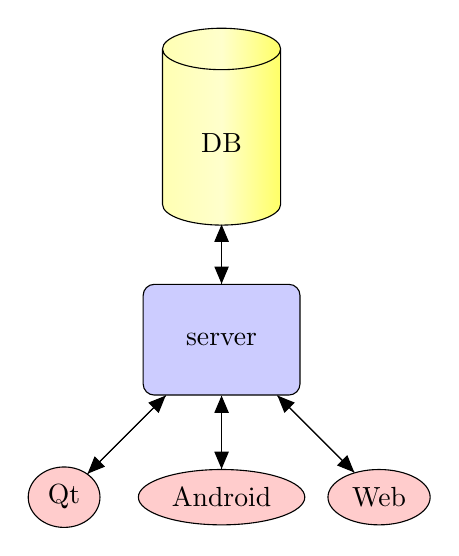
\begin{tikzpicture}[node distance = 2.5cm, auto]
  % Place nodes
  \node [db] (db) {DB};
  \node [block, below of=db] (server) {server};
  
  \node [cloud, below of=server, node distance = 2cm] (client2) {Android};
  \node [cloud, right of=client2, node distance = 2cm] (client1) {Web};
  \node [cloud, left of=client2, node distance = 2cm] (client3) {Qt};

  %pahts
  
  \path [line] (server) -- (db);
  \path [line] (db) -- (server);
  
  \path [line] (client1) -- (server);
  \path [line] (client2) -- (server);
  \path [line] (client3) -- (server);
  \path [line] (server) -- (client1);
  \path [line] (server) -- (client2);
  \path [line] (server) -- (client3);

\end{tikzpicture}
\end{columns}
\end{frame}



%--------------------------------------------------------
\subsection{API Overview}

\begin{frame}[fragile]
\frametitle{API Overview}
\texttt{\color{gray}http://domain.com}\texttt{/api/metamodel}
\texttt{\color{gray}http://domain.com}\texttt{/api/schema}
\texttt{\color{gray}http://domain.com}\texttt{/api/sync}
\texttt{\color{gray}http://domain.com}\texttt{/api/create}

\pad
\pad

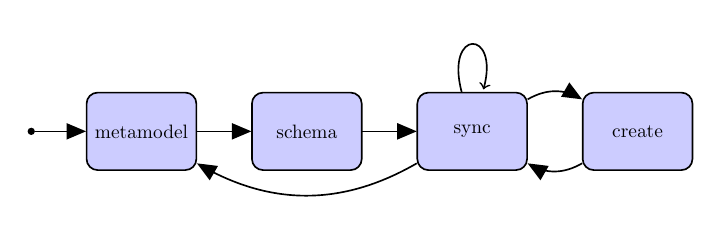
\begin{tikzpicture}[node distance = 3cm, semithick, auto, scale=.7, every node/.style={transform shape}]
  % Place nodes
  \node [dot] (start) {};
  \node [block, right of=start, node distance=2cm] (s1) {metamodel};
  \node [block, right of=s1] (s2) {schema};
  \node [block, right of=s2] (s3) {sync};
  \node [block, right of=s3] (s4) {create};
 
  \path [line] (start) -- node {} (s1) ;
  \path [line] (s1) -- node {} (s2);
  \path [line] (s2) -- node {} (s3);

  \path (s3) edge [loop above] node {} (s3);
  \path (s3) edge [line,bend left] node {} (s1);

  \path (s3) edge [line, bend left] node {} (s4);
  \path (s4) edge [line, bend left] node {} (s3);

\end{tikzpicture}

\end{frame}





%--------------------------------------------------------
\subsection{API Example}
\begin{frame}
\frametitle{API Example}

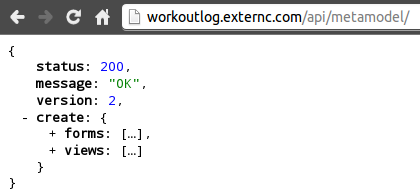
\includegraphics[width=.9\linewidth]{images/metamodel.png} \\
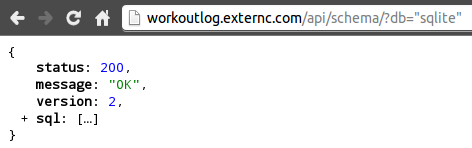
\includegraphics[width=.9\linewidth]{images/schema.png}
\end{frame}




%--------------------------------------------------------
\section{Database Replication}

\begin{frame}
\frametitle{/api/sync: Database replication}
We make use of \textit{metacolumns}: typical SQL columns that are used for some application level purpose.

\begin{columns}[c]
\column{2in}
\scalebox{.8}{
  \begin{tabular}{ l  l  l  l }
  id  & name      & year  & \textit{mod\_ts} \\
  \hline 
  1   & Alice & 4     & \textit{0}        \\
  2   & Bob     & 4     & \textit{10}        \\
  3   & Carol    & 3     & \textit{0}        \\
  4   & Dan      & 4     & \textit{10}        \\
  \end{tabular}
}
\column{2in}
\small
\begin{itemize}
\item The \texttt{mod\_ts} column contains the most recent update on that tuple
\item Allows the server to give clients missing information when supplied with most recent client side \texttt{mod\_ts}
\end{itemize}
\end{columns}
\end{frame}









%--------------------------------------------------------
%\subsection{Implementation}
%
%\begin{frame}
%\frametitle{How to support Synchronization}
%
%\frametitle{Synchronization protocol and API}
%
%There are two simple RESTful function that enable synchronization
%
%\begin{itemize}
%\item \texttt{/api/sync} : Request all tuples on the server that are not present on the client.
%\item \texttt{/api/schema} : Request the SQL that builds the database.
%\end{itemize}
%
%\pad
%
%Normal \texttt{GET} requests can include a representative signature instead. $T$ and $M$ are the concatenation of table names and maximum \texttt{mod\_ts}.
%\begin{itemize}
%\item \textit{$sha1(version + T + M + username + sha1(password))$}
%\end{itemize}
%
%\end{frame}




%--------------------------------------------------------
\subsection{Example}

\begin{frame}
\frametitle{Sample client - server dialog}

\begin{columns}[c]
\column{2in}
Here is a sample conversation between a server and a client who has an out of date schema while attempting to re-sync. \\

\pad

\emph{note:} The application will not require updates for database changes.
\column{2in}
\scalebox{.6}{
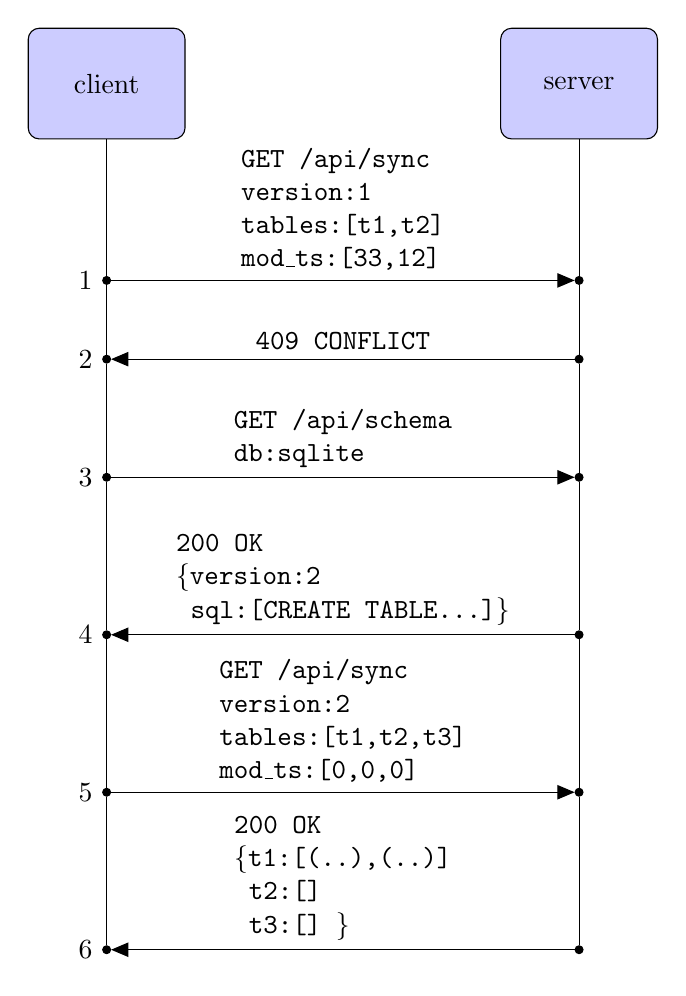
\begin{tikzpicture}[node distance = 2cm, auto]
  % Place nodes
  \node [block] (client) {client};
  \node [block, right of=client, node distance=6cm] (server) {server};
  
  \node [dot, below of=client, node distance=2.5cm, label=180:1] (c1) {};
  \node [dot, below of=server, node distance=2.5cm] (s1) {};
  \path [line] (c1) -- node [above, align=left] {
    \tt\textbf{GET /api/sync} \\ 
    \tt version:1 \\ 
    \tt tables:[t1,t2] \\ 
    \tt mod\_ts:[33,12]}   (s1);
  \path [edge] (client) -- (c1);
  \path [edge] (server) -- (s1);

  \node [dot, below of=c1, node distance=1cm, label=180:2] (c2) {};
  \node [dot, below of=s1, node distance=1cm] (s2) {};
  \path [line] (s2) -- node [above] {\tt\textbf{409 CONFLICT}} (c2);
  \path [edge] (c2) -- (c1);
  \path [edge] (s2) -- (s1);

  \node [dot, below of=c2, node distance=1.5cm, label=180:3] (c3) {};
  \node [dot, below of=s2, node distance=1.5cm] (s3) {};
  \path [line] (c3) -- node [above, align=left] {
    \tt\textbf{GET /api/schema} \\ 
    \tt db:sqlite            } (s3);
  \path [edge] (c2) -- (c3);
  \path [edge] (s2) -- (s3);

  \node [dot, below of=c3, node distance=2cm, label=180:4] (c4) {};
  \node [dot, below of=s3, node distance=2cm] (s4) {};
  \path [line] (s4) -- node [above, align=left] {
    \tt\textbf{200 OK} \\
    \tt\{version:2 \\
    \tt~sql:[CREATE TABLE...]\} } (c4);
  \path [edge] (c3) -- (c4);
  \path [edge] (s3) -- (s4);
    
  \node [dot, below of=c4, node distance=2cm, label=180:5] (c5) {};
  \node [dot, below of=s4, node distance=2cm] (s5) {};
  \path [line] (c5) -- node [above, align=left] {
    \tt\textbf{GET /api/sync} \\ 
    \tt version:2 \\ 
    \tt tables:[t1,t2,t3] \\ 
    \tt mod\_ts:[0,0,0]}   (s5);

  \path [edge] (c5) -- (c4);
  \path [edge] (s4) -- (s5);


  \node [dot, below of=c5, node distance=2cm, label=180:6] (c6) {};
  \node [dot, below of=s5, node distance=2cm] (s6) {};
  \path [line] (s6) -- node [above, align=left] {
    \tt\textbf{200 OK} \\
    \tt \{t1:[(..),(..)] \\
    \tt~t2:[] \\
    \tt~t3:[] \}} (c6);
  \path [edge] (c6) -- (c5);
  \path [edge] (s6) -- (s5);

\end{tikzpicture}
}
\end{columns}


\end{frame}







%--------------------------------------------------------
\subsection{Implementation}

\begin{frame}
\frametitle{How does the mobile client work.}


The entire database is mirrored locally.

\vbox to 30pt{}
\begin{columns}[c]
\column{2in}

\begin{itemize}
\item Only dependent on network for posting changes
\item Faster query times than Window or Cache could ever reach
\item Simple to understand
\end{itemize}

\column{2in}
\scalebox{.65}{% 
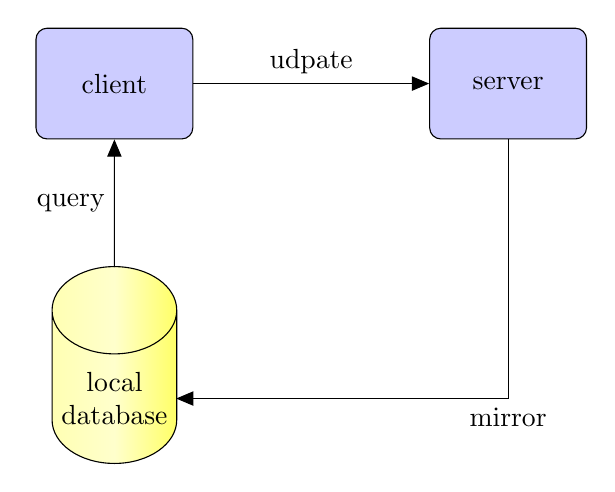
\begin{tikzpicture}[node distance = 2cm, auto]
  % Place nodes
  \node [block] (client) {client};
  \node [block, right of=client, node distance=5cm] (server) {server};
  \node [db, below of=client, node distance=4cm, align=center] (database) {local \\ database};

  % Draw edges
  % Need to align in order to line break
  \path [line] (client) -- node {udpate} (server);
  \path [line] (server) |- node {mirror} (database);
  \path [line] (database) -- node [align=left] {query} (client);
\end{tikzpicture}
}
\end{columns}


\end{frame}


%--------------------------------------------------------

\begin{frame}[fragile]
\frametitle{How does the client know what to request?}


\begin{columns}[c]
\column{2in}
\begin{lstlisting}
[
{"tag":"CAPS05654",
"serial":"000203001056084",
"model":"TCH-17",
"contract number":"none",
"hostname":"USR-Orono1",
"description":"TotalControl17"
},
{"tag":"CAPS05407",
"serial":"72729663",
"model":"7206VXR",
"contract number":"none",
"hostname":"GW-UMF",
"description":"6.SlotChassis"
}
]
\end{lstlisting}
\column{2in}

\begin{lstlisting}
create table Exercises(
  exercise VARCHAR(30) PRIMARY KEY,
  mod_ts DATETIME, 
  deleted INTEGER  
);

create table Sets(
  name VARCHAR(30),
  exercise VARCHAR(30),
  set_num INTEGER ,
  reps_done INTEGER ,
  weight INTEGER ,
  date_done DATE,
  mod_ts DATETIME, 
  deleted INTEGER 
);

\end{lstlisting}

\end{columns}

\end{frame}




%--------------------------------------------------------
\section{Deployment}

\begin{frame}[fragile]
\frametitle{How does deployment work?}

\begin{columns}[c]
\column{1.6in}
Tentatively, a conf file must be filled out. I have made a tool that will download and compile the latest version of Coexist and its clients according to this.
\column{2.5in}
\begin{lstlisting}

; Android stuff
name=Workoutlog
image=logo.png
notification=notification.png
package=com.domain
api=http://domain.com:/api/

; Server stuff
version=1
user=
pass=
db=
host=localhost
dbms=mysql

create_dir=ui 
schema_dir=sql

\end{lstlisting}

\end{columns}


\end{frame}




%--------------------------------------------------------
\section{Future}

\begin{frame}
\frametitle{What needs to be done?}

\begin{itemize}
\item Add more client types (Qt, Desktop Java etc.)
\item Support more client features (i.e. Barcode scanning on mobile clients.)
\item Create tools to automate the configuration.
\end{itemize}

\end{frame}


%--------------------------------------------------------
\section{Thanks}

\begin{frame}
\frametitle{I would like to thank}

My advisor, Sudarshan Chawathe

\end{frame}




%--------------------------------------------------------

\begin{frame}
\frametitle{Authentication}
\begin{itemize}
\item \textit{$sha1(version + T + M + username + sha1(password))$}
\end{itemize}


\end{frame}



%--------------------------------------------------------

\begin{frame}[fragile]
	\center
\frametitle{Handling deletes}
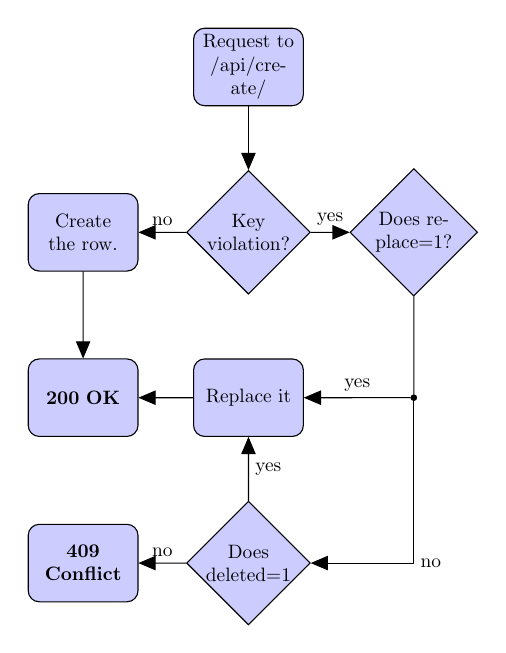
\begin{tikzpicture}[node distance = 3cm, auto, scale=.7, every
	node/.style={transform shape} ]
% Place nodes
\node [block] (request) {Request to /api/create/};
\node [decision, below of=request] (isconflict) {Key violation?};

\node [block, left of=isconflict] (create) {Create the row.};
\node [decision, right of=isconflict] (nocreate) {Does replace=1?};

\node [block, below of=create] (ok) {\textbf{200 OK}};

\node [dot, below of=nocreate] (nocreateDOT) {};

\node [block, left of=nocreateDOT] (replace) {Replace it};
\node [decision, below of=replace] (isreplace) {Does
deleted=1};

\node [block, left of=isreplace] (error) {\textbf{409
Conflict}};

% Draw edges
\path [line] (request) -- (isconflict);
\path [line] (isconflict) -- node [above] {no} (create);
\path [line] (isconflict) -- node [above] {yes}
(nocreate);
\path [line] (create) -- (ok);

\path [edge] (nocreate) -- (nocreateDOT);
\path [line] (nocreateDOT) -- node [above] {yes}
(replace);
\path [line] (replace) -- (ok);

\path [line] (nocreateDOT) |- node [right]
{no} (isreplace);
\path [line] (isreplace) -- node [right]
{yes} (replace);

\path [line] (isreplace) -- node [above]
{no} (error);

\end{tikzpicture}

\end{frame}


\end{document}
